% !TeX encoding = UTF-8
% !TeX TS-program = xelatex
% !TeX engine=xelatex
% !TeX spellcheck = en_GB
% !TeX root = ../Herbstrith-H10_over_AI.tex

\subsubsection{Problems and Turing
machines}

In this section we closely follow the lecture notes on the subject by
\textcite{Mueller2016}.

\begin{defin}
  A \emph{(decision) problem} is a subset of the set of finite
  $\zer$-$\one$-strings $\lbrace \zer, \one \rbrace^*$ including the
  empty string $λ$. We call $\lbrace \zer, \one \rbrace$
  \emph{alphabet} and its elements \emph{bits.}
\end{defin}

One immediate objection against this definition is that not all problems
arise as subsets of these strings. However, such problems $Q$ are
captured up to an encoding.

\[ \enc{\cdot} : Q → \lbrace \zer, \one \rbrace^*\]

We usually do not concern ourselves with the details of this encoding.
However, the encoding should capture the structure of the problem.

\begin{exam}
  Consider the problem of deciding whether a finite simple graph is
  connected or not. If we fix each vertex set to be of the form
  $\lbrace 0, 1, …, n\rbrace$, then the set of all graphs can be encoded
  as the set of the respective adjacency matrices written as a string

  \[b_{00}b_{01} …b_{0n}b_{10}…b_{nn}\]

  of length $(n + 1)^2$, where $b_{ij} = \one$ if and only if the
  vertices $i$ and $j$ are connected.
\end{exam}

\begin{defin}
  A \emph{Turing machine} $\mathbb A$ on the \emph{alphabet}
  $A = \lbrace \sta, \emp, \zer, \one \rbrace$ is a tuple $(S, δ)$,
  where $\sstart, \shalt ∈ S$ is a finite non-empty set, called
  \emph{set of states}, and

  \[δ: S × A → S × A × \lbrace -1, 0, 1 \rbrace\]

  is called \emph{transition function}. If $δ(s, a) = (s', b, m)$, we
  demand that the following axioms are satisfied.

  \begin{thmlist}
  \item
    $a = \sta$ if and only if $b = \sta$.
  \item
    If $a = \sta$, then $m ≠ -1$.
  \item
    If $s = \shalt$, then $s' = \shalt$, $a = b$ and $m = 0$.
  \end{thmlist}
\end{defin}

Informally, we can think of a Turing machine as a device, consisting of a
\emph{work-tape} and a \emph{head}. The work-tape stores all the information in
cells arranged in a consecutive order. Each of these cells contains a letter
from the alphabet.

Let us look at the example of a Turing machine in \cref{fig:Turing machine}.
During the run of the machine the head reads the symbol $\zer$ at the current
position and the machine evaluates the transition function $δ$ at $\zer$ and the
current state $\state{overflow}$. Now assume that

\[ δ(\state{overflow}, \zer) = (\state{return}, \one, -1). \]

We interpret this in the following way. The Turing machine changes its state to
$\state{return}$, the head writes $\one$ in the current cell and moves one cell
to the left. The movement is determined by the last item of the triple
$δ(\state{overflow}, \zer)$, where $-1$ indicates moving to the left, $1$
indicates moving to the right, and $0$ indicates not moving at all.

\begin{figure}
  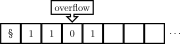
\includegraphics{res/turing_add1_4}
  \caption{A Turing machine}
  \label{fig:Turing machine}
\end{figure}

\begin{defin}
  Let $\mathbb A = (S, δ)$ be a Turing machine. A \emph{configuration}
  of $\mathbb A$ is a triple $(s, j, c) ∈ S × ℕ × A^ℕ$. It reflects
  the current state of $\mathbb A$ the current position of its
  head and the content of its work-tape.
\end{defin}

A configuration of the form $(\shalt, 0, c)$ is called \emph{halting}.
A \emph{start configuration} is of the form $(\sstart, 0, c)$ such
that $c(0) = \sta$ and there exists an $n ∈ ℕ$ such that
$c(i) = \emp$ if and only if $i > n$. This means that in a start
configuration the work-tape reads

\[\sta x_1 x_2 … x_n \emp \emp …\]

It will be very convenient to identify the finite string $x_1…x_n$
with this tape content.

\begin{defin}
  We write $(s, j, c) \vdash_1 (s', j', c')$ and call $(s', j', c')$ a
  \emph{successor configuration} of $(s, j, c)$ if there exists an
  $m ∈ \lbrace -1, 0, 1 \rbrace$ such that

  \begin{itemize}
  \item
    $δ(s, c) = (s', c', m)$,
  \item
    $j' = j + m$, and
  \item
    $c'(ℓ) = c(ℓ)$ for all $ℓ ≠ j$.
  \end{itemize}
\end{defin}

This relation makes the set of all configurations of $\mathbb A$ into
a directed graph. A \emph{run} of $\mathbb A$ on $x$ is a path in
this directed graph starting in the start configuration
$(\sstart, 0, x)$. A run of $\mathbb A$ on $x$ is \emph{halting}
or \emph{complete} if it reaches a halting configuration
$(\shalt, 0, y)$. In this case we write $\mathbb A (x) = y$.

We will denote Turing machines using listings, where the fact that
$δ_\text{delta} (\state{state}, b) = (\state{state'}, c, m)$ is encoded
by

\begin{lstlisting}
delta "state" c = ("state'", c', m)
\end{lstlisting}

Variables \verb+c+ match all possible states or characters in the alphabet
respectively. However, we follow the convention that if an assignment of
variables matches more than one pattern, the first matching pattern is chosen.
This means that
%
\begin{lstlisting}
delta "state" 1 = ("state'", 1, 1)
delta "state" c = ("state''", c, 0)
\end{lstlisting}
%
should be interpreted as
%
\[ δ(s, c) =
  \begin{cases}
    (\state{state'}, \one, 1) & \text{if } s=\state{state} ∧ c = \one\\
    (\state{state''}, c, 0) & \text{if } s=\state{state} ∧ c ≠ \one
  \end{cases}.
\]

See the Appendix of this thesis on how to simulate these Turing machines
using the \emph{Haskell} programming language.

\begin{exam}
    Consider the Turing machine $\mathbb A_\text{add1} = (\lbrace \sstart,
    \shalt, \state{overflow}, \state{return}, \state{error} \rbrace,
    δ_\text{add1})$ that adds $1$ to a (possibly zero-patched) binary
    representation of a natural number $n$. Its transition function is described
    in \cref{lst:add1}. The last line of the program ensures, that $δ$ is a
    complete function, as it matches all remaining pairs of states and
    characters and lets the machine enter the state $\state{error}$.

    The complete run of $\mathbb A_\text{add1}$ on $\one\one\zer\one$ can be
    seen in \cref{fig:complete run}.
\end{exam}

\lstinputlisting[float, frame=tb,
                 caption=A Turing machine adding one to the input string,
                 label=lst:add1]{./listings/add1.hs}

\begin{figure*}
    \begin{subfigure}{.5\textwidth}
        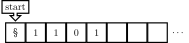
\includegraphics{res/turing_add1_1}
        \caption{$δ(\sstart, \sta) = (s_\text{overflow}, \sta, 1)$}
    \end{subfigure}

    \begin{subfigure}{.5\textwidth}
        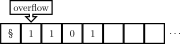
\includegraphics{res/turing_add1_2}
        \caption{$δ(s_\text{overflow}, \one) = (s_\text{overflow}, \one, 1)$}
    \end{subfigure}

    \begin{subfigure}{.5\textwidth}
        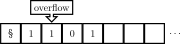
\includegraphics{res/turing_add1_3}
        \caption{$δ(s_\text{overflow}, \one) = (s_\text{overflow}, \one, 1)$}
    \end{subfigure}

    \begin{subfigure}{.5\textwidth}
        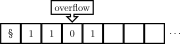
\includegraphics{res/turing_add1_4}
        \caption{$δ(s_\text{overflow}, \zer) = (s_\text{return}, \one, -1)$}
    \end{subfigure}

    \begin{subfigure}{.5\textwidth}
        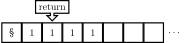
\includegraphics{res/turing_add1_5}
        \caption{$δ(s_\text{return}, \one) = (s_\text{return}, \one, -1)$}
    \end{subfigure}

    \begin{subfigure}{.5\textwidth}
        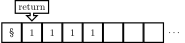
\includegraphics{res/turing_add1_6}
        \caption{$δ(s_\text{return}, \one) = (s_\text{return}, \one, -1)$}
    \end{subfigure}

    \begin{subfigure}{.5\textwidth}
        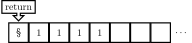
\includegraphics{res/turing_add1_7}
        \caption{$δ(s_\text{return}, \sta) = (s_\text{halt}, \sta, 0)$}
    \end{subfigure}

    \begin{subfigure}{.5\textwidth}
        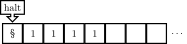
\includegraphics{res/turing_add1_8}
        \caption{$δ(s_\text{halt}, \sta) = (s_\text{halt}, \sta, 0)$}
    \end{subfigure}

    \caption{The complete run of $\mathbb A_\text{add1}$ on $\one\one\zer\one$}
    \label{fig:complete run}
\end{figure*}

\begin{defin}
    Let $\mathbb A$ be a Turing machine.

    \begin{thmlist}
        \item
          $\mathbb A$ \emph{computes} the partial function that maps each
          $x$ with a complete run to $\mathbb A(x)$ and is undefined for all
          other strings.
        \item
          $\mathbb A$ \emph{accepts} all $x$ such that
          $\mathbb A(x) = \one$ and \emph{rejects} them if
          $\mathbb A(x) = \zer$.
        \item
          A partial function on $\lbrace \zer, \one \rbrace^*$ is
          \emph{computable} if there is a Turing machine computing it.
        \item
          A subset of $\lbrace \zer, \one \rbrace^*$, i.e. a
          problem, is \emph{decidable} if there is a Turing machine computing
          its characteristic function.
        \item
          A problem is called \emph{semi-decidable} or \emph{computably
          enumerable} if there is a Turing machine accepting precisely the
          elements of the problem.
    \end{thmlist}
\end{defin}

The last item of the definition above means that a problem is
semi-decidable if there is a Turing machine affirming membership of the
corresponding set but it might not be able to refute membership.

\begin{exam}
    We can encode a natural number $n$

    \begin{exlist}
    \item
      in tally notation
      \begin{align*}
        n & ↦ \underbrace{\one…\one}_{n\text{-times}}, \quad \text{if } n > 0 \\
        0 & ↦ λ
      \end{align*}
    \item
      by its binary representation
      \begin{align*}
          n = 2^k + \sum_{i = 0}^{k-1} b_i 2^i & ↦ b_0…b_{k-1}\one, \quad
              \text{if } n > 0\\
                                             0 & ↦ \zer,
      \end{align*}
      or
    \item
      by a shifted and truncated form of its binary representation
      \begin{align*}
        n = 1 + \sum_{i = 0}^k b_i 2^i & ↦ b_0…b_k, \quad \text{if } n > 0\\
                                     0 & ↦ λ
      \end{align*}

      In other words, $n$ is mapped to the $n$-th string if we order $\lbrace
      \zer, \one \rbrace ^ ℕ$ lexicographically. Following an tradition in
      logics we denote $ℕ$ under this last encoding by $ω$.
    \end{exlist}

    In either case the set obtained by encoding $ℕ$ is easily seen to be
    decidable. In the first case, check that the string contains only copies
    of the bit $\one$. Indeed, this can be achieved by the Turing machine

    \[\mathbb A_\text{tally} =
      ( \lbrace \sstart, \shalt, \scheck, \state{accept}, \state{reject},
        \state{rejectMR}, \state{error} \rbrace, δ)\]

    whose transition function is displayed in \cref{lst:tally encoding}.

    In the second case it suffices to check that the string has length $1$
    or ends in an $\one$, and in the third case every string is accepted.
\end{exam}

\lstinputlisting[float, frame=tb,
                 caption=A Turing machine checking whether the input is tally-encoded,
                 label=lst:tally encoding]{./listings/tally.hs}

Taking another look at the definition of computability, we see that only unary
functions defined on subsets of $ω$, mapping to subsets of $ω$ can be
computable. However, we can easily extend this to functions on multiple
variables, by encoding tuples in $ω \times ω$ by elements of $ω$ in such a way,
that the projections $p_i: \enc{(x_1, x_2)} ↦ x_i$ ($i ∈ \lbrace 0, 1 \rbrace$)
are uniformly computable. This means, we have a bijective pairing function $ω
\times ω → ω$ and Turing machines $\mathbb P_1, \mathbb P_2$ computing $p_1$ or
$p_2$ respectively.

\begin{exam}[Pairing functions]
  \begin{exlist}
    \item A simple pairing function encodes the pair

    \[ (b_1b_2…b_n, c_1c_2…c_m) ∈ ω \times ω\]

    by

    \[ b_1b_1b_2b_2…b_nb_n \zer\one c_1c_2…c_m. \]

  \end{exlist}
\end{exam}

\subsubsection{Halting problem}

One can extend the alphabet of Turing machines by encoding characters
i.e.~assigning bit sequences to them. Very common encodings are
\textsc{ASCII} and \textsc{UTF-8}\footnote{See the Appendix for an
  \textsc{ASCII} encoding table and details on \textsc{UTF-8}.}. Using
either one of these encodings the string `haskell' is encoded as

\begin{lstlisting}
h         a         s         k         e         l         l
0110 1000 0110 0001 0111 0011 0110 1011 0110 0101 0110 1100 0110 1100
\end{lstlisting}

In this way we can encode a Turing machine as the \textsc{UTF-8}-encoding of
its transition function $δ$ written as a string as above. Note that
the set of states can implicitly be deduced from the transition function
as the set of acceptable first arguments of $δ$.

One of the fundamental theorems of theoretical computer science is the
existence of a universal Turing machine.

\begin{thm}
    There exists a Turing machine $\mathbb U$ that computes upon receiving
    the tuple $(\ulcorner \mathbb A \urcorner, x)$ as input, the output of
    Turing machine $\mathbb A$ on $x$ i.e.
    \[ \mathbb U(\ulcorner \mathbb A \urcorner, x) = y \Leftrightarrow \mathbb A (x) = y\]
\end{thm}

A natural question is:

Given a machine $\mathbb A$ and a string $x$. Does $\mathbb A$
halt on $x$?

It is one of the most fundamental results of theoretical computer
science that the halting problem is unsolvable.

\begin{thm}
    The halting problem is undecidable.
\end{thm}
\begin{proof}
    Assume there exists a Turing machine $\mathbb B$ that decides the
    halting problem i.e.~for all Turing machines $\mathbb A$ and all
    strings $x$

    \[ \mathbb B(\enc{\mathbb A}, x) =
    \begin{cases}
      \one  & \text{if } \mathbb A \text{ halts on } x\\
      \zer  & \text{if } \mathbb A \text{ does not halt on } x
    \end{cases}\]

    Now using $\mathbb B$ construct a Turing machine $\mathbb B'$ that
    simulates $\mathbb B(\enc{\mathbb A}, \enc{\mathbb A})$ on its input
    $\enc{\mathbb A}$ and enters an infinite loop if
    $\mathbb B(\enc{\mathbb A}, \enc{\mathbb A}) = \zer$. Expressed more
    formally this means

    \[
      \mathbb B' \text{ halts on } \enc{\mathbb A} ⇔
      \mathbb A \text{ does not halts on } \enc{\mathbb A}.
    \]

    Setting $\mathbb A = \mathbb B'$ yields the desired contradiction.
\end{proof}

For a more detailed proof of this fact and lot more information on computability see \cite{Cooper2004}.
